% !TEX root = root.tex
% 

\documentclass[letterpaper, 10 pt, conference]{ieeeconf}
%\documentclass[a4paper, 10pt, conference]{ieeeconf}

\input{latex_common/preamble.tex}
\input{latex_common/my_tikz.tex}
\usepackage{subfig}

\newcommand{\ocost}{\phi}

\newcommand{\setEcvx}{\mathcal{E}_{\text{cvx}}}
\newcommand{\setIcvx}{\mathcal{I}_{\text{cvx}}}
\newcommand{\setEncvx}{\mathcal{E}_{\text{ncvx}}}
\newcommand{\setIncvx}{\mathcal{I}_{\text{ncvx}}}

\newcommand{\z}{z}
\newcommand{\nz}{n_{\z}}
\renewcommand{\zb}{\bar{z}}
\newcommand{\vc}{\nu}
\newcommand{\vcc}{\sigma}
\newcommand{\tr}{\eta}
\newcommand{\pmet}{\rho}

% convex/non-convex functions
\newcommand{\fc}{g}
\newcommand{\fni}{h}
\newcommand{\fne}{f}
\newcommand{\fnib}{\bar{\fni}}
\newcommand{\fneb}{\bar{\fne}}

\IEEEoverridecommandlockouts                              % This command is only needed if                                                         % you want to use the \thanks command

\overrideIEEEmargins                                      % Needed to meet printer requirements.

%In case you encounter the following error:
%Error 1010 The PDF file may be corrupt (unable to open PDF file) OR
%Error 1000 An error occurred while parsing a contents stream. Unable to analyze the PDF file.
%This is a known problem with pdfLaTeX conversion filter. The file cannot be opened with acrobat reader
%Please use one of the alternatives below to circumvent this error by uncommenting one or the other
%\pdfobjcompresslevel=0
%\pdfminorversion=4

% See the \addtolength command later in the file to balance the column lengths
% on the last page of the document

% The following packages can be found on http:\\www.ctan.org
%\usepackage{graphics} % for pdf, bitmapped graphics files
%\usepackage{epsfig} % for postscript graphics files
%\usepackage{mathptmx} % assumes new font selection scheme installed
%\usepackage{times} % assumes new font selection scheme installed
%\usepackage{amsmath} % assumes amsmath package installed
%\usepackage{amssymb}  % assumes amsmath package installed

\title{\LARGE \bf Title
}


\author{Taylor P. Reynolds and Mehran Mesbahi% <-this % stops a space
\thanks{*This research has been supported by XXX}% <-this % stops a space
\thanks{The authors are with the W.E. Boeing Department of Aeronautics and Astronautics,
        University of Washington, Seattle, WA, USA.
        {\tt\small \{tpr6,mesbahi\}@uw.edu}}%
% \thanks{$^{2}$Bernard D. Researcher is with the FacultyDepartment of Electrical Engineering, Wright State University,
%         Dayton, OH 45435, USA
%         {\tt\small b.d.researcher@ieee.org}}%
}

\begin{document}

\maketitle
\thispagestyle{empty}
\pagestyle{empty}


%%%%%%%%%%%%%%%%%%%%%%%%%%%%%%%%%%%%%%%%%%%%%%%%%%%%%%%%%%%%%%%%%%%%%%%%%%%%%%%%
\begin{abstract}

abstract.

\end{abstract}


%%%%%%%%%%%%%%%%%%%%%%%%%%%%%%%%%%%%%%%%%%%%%%%%%%%%%%%%%%%%%%%%%%%%%%%%%%%%%%%%
\section{INTRODUCTION}\label{sec:intro}

The point of this paper is to communicate the ``creeping phenonmenon'' that occurs in sequential convex programming algorithms that are designed a certain way. It seems to be a fundamental limitation of a certain class of algorithms. 

\begin{itemize}
\item what is the purpose of the paper?
\item why is this important, and how is it useful?
\end{itemize}

\section{SEQUENTIAL CONVEX PROGRAMMING}\label{sec:scp}

\begin{itemize}
\item provide an overview of SCP methods, similar to a condensed version of CSM.
\item provide a generalized algorithmic framework for the class of algorithms susceptible to the creeping phenomenon.
\end{itemize}
% only go so far as to define the linear and nonlinear costs as "original cost" plus "feasibility measure". 

Consider the following optimization problem
\begin{subequations}\label{eq:nlp}
\begin{align}
\min_z &\quad \ocost(\z) &&\null \label{eq:nlp_a} \\
\text{s.t.} &\quad \fc_i(\z) \leq 0, &&\quad i \in \setIcvx \label{eq:nlp_b}\\
&\quad \fni_i (\z) \leq 0, &&\quad i \in \setIncvx \label{eq:nlp_c} \\
&\quad \fne_j(\z) = 0, &&\quad j \in \setEncvx \label{eq:nlp_d}
\end{align}
\end{subequations}
where $\z\in\real^{\nz}$, $\setIcvx = \{1,\ldots,m_i\}$, $\setIncvx=\{m_i+1,\ldots,m_i+n_i\}$ represent the indices of the convex and non-convex inequality constraints and $\setEncvx=\{1,\ldots,n_e\}$ represents the indices of non-convex equality constraints. We shall assume that the cost function $\ocost$ is convex, and that each $\fni_i$ and $\fne_j$ are at least once differentiable almost everywhere. To simplify the notation, we assume that any convex equality constraint is represented by a pair of convex inequality constraints. Problem~\eqref{eq:nlp} is typically refered to as a nonlinear programming problem, but herein we shall refer to it as the original non-convex optimization problem (or simple the original problem). While there exist general purpose solvers that are able to solve the original problem (see, e.g.,~\cite{Gill1981,NocedalWright}), a current trend is to seek solutions by using iterative schemes that are based on convex optimization. 

The barrier to directly applying convex optimization methods is of course the set of non-convex constraints~\eqref{eq:nlp_c} and~\eqref{eq:nlp_d}. Sequential convex programming methods approximate each of these constraints with a convex function of the solution variable, and iteratively update the approximations based on the solution of the resulting convex program. In this way, the original problem is transformed into a sequence of convex subproblems. Each convex approximation is computed using a reference solution, $\zb$, and takes the form
\begin{subequations}\label{eq:cvx_approximation_general}
\begin{align}
\fnib_i(\z,\zb) \leq 0, \quad i\in\setIncvx, \label{eq:cvx_approximation_general_ineq} \\
\fneb_j(\z,\zb) = 0, \quad j\in\setEncvx. \label{eq:cvx_approximation_general_eq}
\end{align}
\end{subequations}
There are several choices for $\fnib_i$: first- or second-order Taylor series approximations, inner convex approximations, or any other convex function that locally approximates the non-convex $h_i$. The $\fneb_j$ on the other hand must be affine functions of $\z$. The approximations $\fnib_i$ and $\fneb_j$ are therefore inherently local; their accuracy decreases as $\|\z-\zb\|$ increases. As a separate issue, consider the possible scenario where $\ocost$ and each $g_i$ are linear functions, and we choose each $\fnib_i$ to be a first-order approximation (i.e., the linearization of $\fni_i$ around $\zb$). In this case, the resulting optimization problem is unbounded below, a phenomenon refered to as \textit{artificial unboundedness}. To address the local nature of the approximations~\eqref{eq:cvx_approximation_general} and to avoid artificial unboundedness, we add a \textit{trust region} constraint of the form
\begin{equation}
\| \z - \zb \|_q \leq \tr,
\label{eq:trust_region}
\end{equation}
where $q=\{1,\,2,\,\infty\}$ and $\tr\in\realpp$ is a positive \textit{trust region radius}. Now we may formulate the following convex approximation to Problem~\eqref{eq:nlp}:
\begin{subequations}\label{eq:cvx_tr}
\begin{align}
\min_z &\quad \ocost(\z) &&\null \label{eq:cvx_tr_a} \\
\text{s.t.} &\quad \fc_i(\z) \leq 0, &&\quad i\in\setIcvx \label{eq:cvx_tr_b} \\
&\quad \fnib_i(\z,\zb) \leq 0, &&\quad i\in\setIncvx \label{eq:cvx_tr_c}\\
&\quad \fneb_j(\z,\zb) = 0, &&\quad j\in\setEncvx \label{eq:cvx_tr_d} \\
&\quad \| \z - \zb \|_q \leq \tr  &&\null \label{eq:cvx_tr_e}
\end{align}
\end{subequations}
Problem~\eqref{eq:cvx_tr} is a convex program. However, directly solving Problem~\eqref{eq:cvx_tr} has proved difficult in several previous studies \todo{add studies}. In particular, Problem~\eqref{eq:cvx_tr} is susceptible to \textit{artificial infeasibility} that stems from two probable causes. First, the approximations~\eqref{eq:cvx_tr_c}~\eqref{eq:cvx_tr_d} and trust region~\eqref{eq:cvx_tr_e} can be incompatible, in the sense that $\mathcal{F}_1 = \{\z\,|\,\eqref{eq:cvx_tr_c},~\eqref{eq:cvx_tr_d}\text{ and }\eqref{eq:cvx_tr_d}\text{ are satisfied}\} = \emptyset$. 
%This may occur when the reference $\zb$ is further than a distance $\tr$ from the set $\{\z\,|\,g_i(\z)\leq0,~i\in\setIcvx\}$ under the $q$-norm. 
Second, the constraints~\eqref{eq:cvx_tr_b},~\eqref{eq:cvx_tr_c} and~\eqref{eq:cvx_tr_d} can be incompatible, in the sense that $\mathcal{F}_2 = \{\z\,|\,\eqref{eq:cvx_tr_b}\text{ and }\eqref{eq:cvx_tr_c}~\eqref{eq:cvx_tr_d}\text{ are satisfied}\}=\emptyset$. Illustrations of these two cases are shown graphically in Figure~\ref{fig:artificial_infeas}. Artificial infeasibility can be avoided by adding so-called \textit{virtual control} to~\eqref{eq:cvx_tr_c}:
\begin{subequations}\label{eq:virtual_control}
\begin{align}
\fnib_i(\z,\zb) - \vcc_i \leq 0 \\
\fneb_j(\z,\zb) - \vc_j = 0
\end{align}
\end{subequations}
where $\vcc_i > 0$. The vectors $\vcc\in\real^{n_i}$ and $\vc\in\real^{n_e}$ are added as solution variables, and the resulting augmented convex program is%
\begin{figure}
\centering
\subfloat[$\mathcal{F}_1 = \emptyset$.]{% !TEX ROOT = ../root.tex

\begin{tikzpicture}
\tikzmath{
	\hx=1.75; \hy=1.75; \hyy=-1.25;
	\cx=0.70; \cy=0.95;
	\dds=0.035;
	\xintrsct=\cx;
	\xright=0.85;
	\slp=0.5;
}
\tikzstyle{every node}=[font=\footnotesize]

% draw axes
\draw[->] (0,\hyy) -- (0,\hy) node[anchor=east] {$z_2$};
\draw[<->] (-\hx,0) -- (\hx,0) node[anchor=north] {$z_1$};
\foreach \x in {-1,-0.5,0.5,1} \draw[] (\x,-\dds) -- (\x,\dds);
\foreach \y in {-1,-0.5,0.5,1} \draw[] (-\dds,\y) -- (\dds,\y);
% draw trust region
\draw[densely dashed,red,fill=red,fill opacity=0.2] (\cx,\cy) circle (0.4);
\node[anchor=south,red,name=tr] at (\cx+0.3,\cy+0.65) {$\| \z - \zb \|_2 \leq \tr$};
\draw[] (tr.south) to[out=-90,in=90] (\cx,\cy+0.45);
% draw zb
\filldraw[black] (\cx,\cy) circle (1.5pt) node[anchor=south east,yshift=-0.1cm] {$\zb$};
% draw ncvx constraint
\draw[thick,domain=-1:\hy,smooth,variable=\x,blue] plot ({\x},{\slp*\x*\x});
\node[anchor=south,name=ncvx,blue] at (-1,0.5) {$\fne_1(\z)=0$};
% draw cvx linearization
\draw[thick,domain=-0.25:\hy,smooth,variable=\x,dashed,red] plot ({\x},{2*\slp*\xintrsct*\x-\slp*\xintrsct*\xintrsct});
\node[anchor=north,name=cvx,red] at (\cx+0.15,-0.25) {$\fneb_1(\z,\zb)=0$};

\end{tikzpicture}} \hfil
\subfloat[$\mathcal{F}_2 = \emptyset$]{% !TEX ROOT = ../root.tex

\begin{tikzpicture}
\tikzmath{
	\hx=1.75; \hy=1.75; \hyy=-1.25;
	\cx=0.40; \cy=0.5;
	\dds=0.035;
	\xintrsct=\cx;
	\xright=0.85;
	\slp=0.5;
	\bx=1.5; \mMm=-0.15; \bBb=1;
	\cXx=0.2; \dXx=0.06;
}
\tikzstyle{every node}=[font=\footnotesize]

% draw axes
\draw[->] (0,\hyy) -- (0,\hy) node[anchor=east] {$z_2$};
\draw[<->] (-\hx,0) -- (\hx,0) node[anchor=north] {$z_1$};
\foreach \x in {-1,-0.5,0.5,1} \draw[] (\x,-\dds) -- (\x,\dds);
\foreach \y in {-1,-0.5,0.5,1} \draw[] (-\dds,\y) -- (\dds,\y);
% draw trust region
\draw[densely dashed,red,fill=red,fill opacity=0.2] (\cx,\cy) circle (0.5);
% \node[anchor=south,red,name=tr] at (\cx+0.3,\cy+0.65) {$\| \z - \zb \|_2 \leq \tr$};
% \draw[] (tr.south) to[out=-90,in=90] (\cx,\cy+0.45);
% draw zb
\filldraw[black] (\cx,\cy) circle (1.5pt) node[anchor=south east,yshift=-0.1cm] {$\zb$};
% draw ncvx constraint
\draw[thick,domain=-1:\hy,smooth,variable=\x,blue] plot ({\x},{\slp*\x*\x});
\node[anchor=south,name=ncvx,blue] at (-1,0.5) {$\fne_1(\z)=0$};
% draw cvx linearization
\draw[thick,domain=-0.5:\hy,smooth,variable=\x,dashed,red] plot ({\x},{2*\slp*\xintrsct*\x-\slp*\xintrsct*\xintrsct});
\node[anchor=north,name=cvx,red] at (-0.5,-0.25) {$\fneb_1(\z,\zb)=0$};
% draw inequality g1
\draw[thick,domain=-0.5:\hy,smooth,variable=\x,darkgreen] plot ({\x},{\mMm*\x+\bBb});
\draw[darkgreen,->] (\cXx-0.0707,\mMm*\cXx+\bBb+0.0707) -- ++(\dXx,-\dXx/\mMm);
\node[anchor=south,darkgreen] at (-1,1.1) {$\fc_1(\z) \leq 0$};
% draw inequality g2
\draw[thick,darkgreen] (\bx,-1) -- (\bx,1.5);
\draw[darkgreen,->] (\bx-0.1,-0.8) -- ++(-0.4,0); 
\node[anchor=north,darkgreen] at (\bx,-1) {$\fc_2(\z)\leq0$};


\end{tikzpicture}}
\caption{A depiction of the two causes of artificial infeasibility.}
\label{fig:artificial_infeas}
\end{figure}
\begin{subequations}\label{eq:cvx_apprx}
\begin{align}
\min_{\z,\vcc,\vc} &\quad \ocost(\z) + \lambda P(\vcc,\vc) &&\null \label{eq:cvx_apprx_a} \\
\text{s.t.} &\quad \fc_i(\z) \leq 0, &&\quad i\in\setIcvx \label{eq:cvx_apprx_b} \\
&\quad \fnib_i(\z,\zb) - \vcc_i \leq 0, &&\quad i\in\setIncvx \label{eq:cvx_apprx_c}\\
&\quad \fneb_j(\z,\zb) - \vc_j = 0, &&\quad j\in\setEncvx \label{eq:cvx_apprx_d} \\
&\quad \|\z-\zb\|_q \leq \tr &&\null  \label{eq:cvx_apprx_e}
\end{align}
\end{subequations}
where $P : \real^{n_e}\times\real^{n_i} \rightarrow \realpp$ is a positive-definite penalty function and $\lambda>0$ is a user-selected weight. Typically $\lambda \gg 1$ to limit the use of virtual control only to cases when it is required to avoid artificial infeasibility.

We shall refer to a solution to Problem~\eqref{eq:cvx_apprx} as an \textit{iterate}, and denote it by $(\z^*,\vcc^*,\vc^*)$. Sequential convex programming algorithms iteratively solve Problem~\eqref{eq:cvx_apprx} and use resulting iterate to update $\zb$. Moreover, the iterate $(\z^*,\vcc^*,\vc^*)$ can be used to update the value of $\tr$, based on some assessment of the accuracy of the approximation in~\eqref{eq:cvx_approximation_general}. The resulting sequence of solutions $\zb$ approaches a locally optimal solution of~\eqref{eq:nlp} under certain conditions and problem assumptions. There have been numerous papers that study the convergence properties of these algorithms, offering conditions/assumptions under which convergence is guaranteed to various flavors of minima~\todo{add citations}. This paper does not discuss \textit{whether} convergence is achieved or at what rate, but instead looks at an implicit property of SCP type algorithms that use the validity of the approximations to update the trust region size.

\subsection{Trust Region Updates}\label{subsec:tr_updates}

Most sequential convex programming methods use a dynamically sized trust region. The size of $\tr$ is updated with each iteration according to a set of rules that are specified by the designer. These rules are designed to facilitate formal convergence proofs, and makes use of a performance metric that is based on $(\z^*,\vcc^*,\vc^*)$ to do so. The performance metric can be thought of as a function that provides key feedback to the iterative process and guides convergence. To introduce a few common performance metrics, we first define the following functions
\begin{subequations}\label{eq:scp_costs}
\begin{align}
J(\z) &= \ocost(\z) + \lambda P\big( \fni(\z),\,\fne(\z) \big) \label{eq:scp_costs_nl}\\
L(\z) &= \ocost(\z) + \lambda P\big( \fnib(\z,\zb),\,\fneb(\z,\zb) \big) \label{eq:scp_costs_l}
\end{align}
\end{subequations}
where $\fni(\z) \in \real^{n_i}$ and $\fne(\z)\in\real^{n_e}$ are the concatenations of the non-convex constraints from the original problem~\eqref{eq:nlp_c}, and similarly for $\fnib(\z,\zb)$ and $\fneb(\z,\zb)$. The cost functions in~\eqref{eq:scp_costs} can be thought of as measuring the optimality (via $\ocost$) and the feasibility (via $P(\cdot,\cdot)$) of a candidate solution. The measure of feasibility is weighted by $\lambda$. The function~\eqref{eq:scp_costs_nl} measures this weighted cost with respect to the original non-convex problem~\eqref{eq:nlp}, while the function~\eqref{eq:scp_costs_l} measures the same weighted cost with respect to the approximated convex problem~\eqref{eq:cvx_apprx}. 

We now introduce two commonly used performance metrics. The first is simply the \textit{relative error}
\begin{equation}
\pmet = \frac{J(\z^*) - L(\z^*)}{L(\z^*)},
\label{eq:pmet_rel_error}
\end{equation}
which measures how close the original non-convex and approximated convex weighted costs are. The ideal value of the relative error is zero. Another performance metric is the \textit{relative decrement} defined as
\begin{equation}
\pmet = \frac{J(\zb) - J(\z^*)}{J(\zb) - L(\z^*)},
\label{eq:pmet_rel_decrement}
\end{equation}
which measures how well the convex approximation predicts the decrease in the original non-convex weighted cost. The ideal value of the relative decrement is one. Once chosen\footnote{We stress that the choice of performance metric is not arbitrary, but is tied to the use of a specific algorithm. The two possibilities presented here are abstract representations of performance metrics used by algorithms in the literature.}, the scalar-valued performance metric $\pmet$ is used to grow, shrink, or maintain the size of the trust region radius. Crucially, it is also used to reject a solution $\z^*$ in certain cases, which means the same convex approximation is kept but the trust region is shrunk, and the convex problem is re-solved. 

To decide which case we are in for a given iteration (accept/reject, shrink/keep/grow), the user defines three real numbers $\pmet_0,\,\pmet_1,\,\pmet_2\in(0,1)$ that split the real number line into up to four segments. The value of $\pmet$ places each iterate in one of these four segments, and the trust region and reference solution are updated according to the rules in Figure~\ref{fig:scp_updates}. The constants $\alpha,\beta >1$ are the shrink and growth rates, respectively, and are chosen by the designer. 

\begin{figure*}
\centering
% !TEX ROOT = ../root.tex

\begin{tikzpicture}
\tikzmath{
	\cx=0; \cy=0; \wdt=2.5; \hgt=2;
	\dx=0.25; \dxx=0.7;
	\cxx=\cx+\wdt+\dx; 
	\cxxx=\cxx+\wdt+\dx;
	\civ=\cxxx+\wdt+\dx;
	\Rly=\cy-0.5*\hgt-2*\dx;
	\cyy=\Rly-2.5*\dx;
	\cyyy=\Rly+2.5*\dx;
}
\tikzstyle{every node}=[font=\small]

% NUMBER LINE
\begin{scope}[shift={(0,\Rly)}]
% rho_0
\draw[thick,dashed] (\cx+0.5*\wdt+0.5*\dx,6*\dx) -- (\cx+0.5*\wdt+0.5*\dx,-6*\dx) node[anchor=south,pos=0] {$\rho_0$};
% rho_1
\draw[thick,dashed] (\cxx+0.5*\wdt+0.5*\dx,6*\dx) -- (\cxx+0.5*\wdt+0.5*\dx,-6*\dx) node[anchor=south,pos=0] {$\rho_1$};
% rho_2
\draw[thick,dashed] (\cxxx+0.5*\wdt+0.5*\dx,6*\dx) -- (\cxxx+0.5*\wdt+0.5*\dx,-6*\dx) node[anchor=south,pos=0] {$\rho_2$};
% reals
\draw[ultra thick,<->] (\cx-0.5*\wdt-2*\dx,0) -- (\civ+0.5*\wdt+2*\dx,0) node[anchor=west] {\Large $\real$};
\end{scope}

%% TOP TEXT
\node[anchor=south] at (\cx,\cy-\dx) {$\pmet < \pmet_0$};
\node[anchor=south] at (\cxx,\cy-\dx) {$\pmet \in [\pmet_0,\pmet_1)$};
\node[anchor=south] at (\cxxx,\cy-\dx) {$\pmet\in[\pmet_1,\pmet_2)$};
\node[anchor=south] at (\civ,\cy-\dx) {$\pmet \geq \pmet_2$};

%% TOP BOXES
% Case 1
\pane{\cx}{\cyy}{0}{\wdt}{0.5*\hgt}{0.2}{draw,color=red!50!white,fill=red!10!white}
\node[] at (\cx,\cyy) {\begin{tabular}{l}
$\tr \leftarrow \tr / \alpha $ \\
$\zb \leftarrow \zb$ 
\end{tabular}};

% Case 2
\pane{\cxx}{\cyy}{0}{\wdt}{0.5*\hgt}{0.2}{draw,color=yellow!70!black,fill=yellow!10!white}
\node[] at (\cxx,\cyy) {\begin{tabular}{l}
$\tr \leftarrow \tr / \alpha$ \\
$\zb \leftarrow \z^*$ 
\end{tabular}};

% Case 3
\pane{\cxxx}{\cyy}{0}{\wdt}{0.5*\hgt}{0.2}{draw,color=green!50!white!80!black,fill=green!10!white}
\node[] at (\cxxx,\cyy) {\begin{tabular}{l} 
$\tr \leftarrow \tr$ \\
$\zb \leftarrow \z^*$ 
\end{tabular}};

% Case 4
\pane{\civ}{\cyy}{0}{\wdt}{0.5*\hgt}{0.2}{draw,color=green!50!white!80!black,fill=green!10!white}
\node[] at (\civ,\cyy) {\begin{tabular}{l}
$\tr \leftarrow \beta \tr$ \\
$\zb \leftarrow \z^*$
\end{tabular}};

%% BOTTOM BOXES
% Case 1
\pane{\cx}{\cyyy}{0}{\wdt}{0.5*\hgt}{0.2}{draw,color=green!50!white!80!black,fill=green!10!white}
\node[] at (\cx,\cyyy) {\begin{tabular}{l}
$\tr \leftarrow \beta \tr $ \\
$\zb \leftarrow \z^*$ 
\end{tabular}};

% Case 2
\pane{\cxx}{\cyyy}{0}{\wdt}{0.5*\hgt}{0.2}{draw,color=green!50!white!80!black,fill=green!10!white}
\node[] at (\cxx,\cyyy) {\begin{tabular}{l}
$\tr \leftarrow  \tr$ \\
$\zb \leftarrow \z^*$ 
\end{tabular}};

% Case 3
\pane{\cxxx}{\cyyy}{0}{\wdt}{0.5*\hgt}{0.2}{draw,color=yellow!70!black,fill=yellow!10!white}
\node[] at (\cxxx,\cyyy) {\begin{tabular}{l}
$\tr \leftarrow \tr / \alpha$ \\
$\zb \leftarrow \z^*$ 
\end{tabular}};

% Case 4
\pane{\civ}{\cyyy}{0}{\wdt}{0.5*\hgt}{0.2}{draw,color=red!50!white,fill=red!10!white}
\node[] at (\civ,\cyyy) {\begin{tabular}{l}
$\tr \leftarrow \tr / \alpha$ \\
$\zb \leftarrow \zb$
\end{tabular}};

%% LEFT TEXT
\node[text width=2cm, anchor=east, align=right] at (\cx-0.5*\wdt-2*\dx,\cyy) {\textit{Rel.~decrement}};
\node[text width=2cm, anchor=east, align=right] at (\cx-0.5*\wdt-2*\dx,\cyyy) {\textit{Rel.~error}};

\end{tikzpicture}
\caption{Update rules for two different performance metrics of a general sequential convex programming algorithm.}
\label{fig:scp_updates}
\end{figure*}

We now make a brief technical comment before proceeding. First, the denominators in~\eqref{eq:pmet_rel_error} and~\eqref{eq:pmet_rel_decrement} must be verified to be non-zero before computing the value of $\pmet$. In the case of~\eqref{eq:pmet_rel_error}, a sufficient condition to avoid this is $\ocost(\z)>0$ for all feasible $\z$. In the case of~\eqref{eq:pmet_rel_decrement}, a zero denominator actually implies that the iterations can be terminated, since $L(\z^*) \leq L(\zb) = J(\zb)$ (note that this implies the denominator is always nonnegative). If $J(\zb)-L(\z^*)=0$, then the optimal solution found by solving~\eqref{eq:cvx_apprx} is exactly the reference solution, and the iterations may be stopped. Therefore for either performance metric, divide-by-zero conditions can be avoided.   

\section{THE CREEPING PHENOMENON}

Intuition would support the claim that a dynamically sized trust region would allow an SCP algorithm to take larger steps in regions where the convex approximation is the most accurate. In this section we demonstrate that actually the opposite can happen: dynamic trust regions can cause SCP algorithms to make \textit{slow} progress even when the convex approximation is quite accurate. This is not a universal phenonmenon in the sense that it applies equally to all problem scenarios. Rather, intrinsic properties of the original non-convex constraints~\eqref{eq:nlp_c} and the methods used to convexify them can make one problem more susceptible to this phenomenon than others. We will explore this behavior for each of the performance metrics defined in~\sref{subsec:tr_updates} separately.

\subsection{Relative Error}\label{subsec:creep_rel_err}

We introduce the notion of internal resistance by studying algorithms that use the relative error~\eqref{eq:pmet_rel_error} as the metric with which to update the reference and trust region radius. From Figure~\ref{fig:scp_updates}, the algorithm will reject the current step if $\pmet>\pmet_2$, where $\pmet_2<1$ is a user-defined value. It is enough for the current discussion to assume that $\pmet_2=1$, so that subsequent results are sufficient for any chosen value of $\pmet_2$ during implementation. In order that an iterate be accepted, we must then have
\begin{equation}
\frac{J(\z^*) - L(\z^*)}{L(\z^*)} < 1 \quad \Rightarrow \quad  J(\z^*) < 2 L(\z^*).
\label{eq:rel_err_accept}
\end{equation} 
Using~\eqref{eq:scp_costs} this can be rewritten as
\begin{equation}
P\big( \fni(\z^*),\,\fne(\z^*) \big) < \frac{\phi(\z^*)}{\lambda} + 2 P\big( \fnib(\z^*,\zb),\,\fneb(\z^*,\zb) \big).
\label{eq:rel_err_accept_2}
\end{equation}
What~\eqref{eq:rel_err_accept_2} says is that in order for a step to be accepted, the degree to which the iterate $\z^*$ is infeasible for the original non-convex problem must be bounded by the right hand side. If inequality~\eqref{eq:rel_err_accept_2} is violated, we find ourselves in the top-right case in Figure~\ref{fig:scp_updates}: the iterate $\z^*$ is rejected, the trust region is shrunk by an amount $\alpha$ and the problem is resolved. The inequality~\eqref{eq:rel_err_accept_2} can also be interpreted as saying that the infeasibility of all accepted iterates with respect to the original non-convex problem is bounded from above by the sum of the (weighted) original cost and twice the amount of infeasibility in the convex approximation. 

Loosely speaking, the problem of internal resistance appears when there is sufficient curvature in the set of non-convex functions $h$ that is not captured by the approximations $\fnib(\z,\zb)$ or $\fneb(\z,\zb)$. In this case, satisfaction of the convex constraints~\eqref{eq:virtual_control} implies that $P\big(\fni(\z^*),\,\fne(\z^*)\big)$ can be large, and thus the inequality~\eqref{eq:rel_err_accept_2} is violated. This can happen quite easily when, for example, $\fne(\z)$ has a large Lipschitz constant in the set defined by the trust region, and the affine approximation $\fneb_i(\cdot,\zb)$ cannot sufficient capture the the curvature. We provide a specific example of this in~\sref{subsec:toy_example}.

\subsection{Relative Decrement}\label{subsec:crepp_rel_dec}

Algorithms that use the relative decrement as the metric with which to update the reference and trust region size experience the problem internal resistance in a slightly different way. Internal resistance will only arise when the reference is \textit{feasible} (or nearly so) for the original non-convex problem. In this case, we have $P\big(\fni(\z),\,\fne(\z)\big)=0$. To see why, first recall that the denominator in~\eqref{eq:pmet_rel_decrement} is always nonnegative, and that an iterate may be rejected when $\pmet<\pmet_0$ for $\pmet_0>0$. Similar to the relative error case, we shall assume that $\pmet_0=0$ so that the following results are sufficient for any chosen value. If $\pmet_0=0$, then according to the rules in Figure~\ref{fig:scp_updates} an iterate will only accepted if the \textit{numerator} of~\eqref{eq:pmet_rel_decrement} is strictly positive. Hence for an accepted step we have
\begin{subequations}\label{eq:rel_dec_bound}
\begin{gather}
J(\zb) - J(\z^*) > 0 \label{eq:rel_dec_bound_a}\\
\ocost(\zb) - \ocost(\z^*) - \lambda P\big( \fni(\z^*),\,\fne(\z^*) \big) > 0 \label{eq:rel_dec_bound_b}\\
 \frac{\ocost(\zb) - \ocost(\z^*)}{\lambda}  > P\big( \fni(\z^*),\,\fne(\z^*) \big) \label{eq:rel_dec_bound_c}
\end{gather}
\end{subequations}
which says that the degree to which the iterate $\z^*$ is infeasible for the original non-convex problem is bounded by the (weighted) reduction in original cost. If inequality~\eqref{eq:rel_dec_bound_c} is violated, we find ourselves in the bottom-left case in Figure~\ref{fig:scp_updates}: the iterate will be rejected, the trust region shrunk, and the problem is resolved. 

\begin{remark}
The inequality~\eqref{eq:rel_dec_bound_b} also illuminates the fact that if the reference $\zb$ is feasible for the original non-convex problem, then an accepted iterate must (strictly) decrease the original cost. This is due to the fact that $\lambda>0$ and $P(\cdot,\cdot)$ is positive definite.
\end{remark}

Since $\zb$ is feasible for the original problem, we know that actually $\zb$ is a feasible point for Problem~\eqref{eq:cvx_tr} as well (the convex approximation with no virtual control). Thus the optimal solution of Problem~\eqref{eq:cvx_apprx} will not use any virtual control provided that $\lambda$ is large enough\footnote{There exists a non-empty feasible set that uses no virtual control, solutions that are not in this set necessarily increase the cost for large values of $\lambda$.}. The solution $\z^*$ will therefore satisfy $\fnib(\z^*,\zb)\leq 0$ and $\fneb(\z^*,\zb)=0$. If either $\fnib(\cdot,\zb)$ (resp.~$\fneb(\cdot,\zb)$) does not adequately capture the behavior of $\fni(\cdot)$ (resp.~$\fne(\cdot)$), then inequality~\eqref{eq:rel_dec_bound_c} is likely to be violated. This implies that for a given set of non-convex functions $\fni(\cdot)$ and $\fne(\cdot)$, for every feasible $\zb$ there is a \textit{maximum trust region size} that is implicitly defined by the method used to ``convexify'' the original problem and the largest achievable reduction in cost (weighted by $1/\lambda$). For $\lambda\gg1$ the maximum trust region size such that~\eqref{eq:rel_dec_bound_c} is satisfied can be small, causing the algorithm to take small incremental steps that are each nearly feasible for the original non-convex problem. This is depicted in Figure~\todo{add fig} and is the essence of what we refer to as internal resistance.

\subsection{A Simple Example}\label{subsec:toy_example}

This section provides a simple example that exhibits the crawling phenomenon. Consider the following optimization problem in the variable $\z=(z_1,z_2)\in\real^2$
\begin{subequations}\label{eq:toy_prob}
\begin{align}
\min_{\z} &\quad z_1+z_2 \label{eq:toy_prob_a}\\
\text{s.t.} &\quad \fc_1(\z) = -z_2 - \tfrac{4}{3} z_1 - \tfrac{2}{3} \leq 0 \label{eq:toy_prob_b}\\
&\quad \fc_2(\z) = \z - 2 \leq 0 \label{eq:toy_prob_c}\\
&\quad \fc_3(\z) = -\z - 2 \leq 0 \label{eq:toy_prob_d}\\
&\quad \fne_1(\z) = z_2 - z_1^4 + 2z_1^3 - 1.2z_1^2 - 2z_1 = 0 \label{eq:toy_prob_e}
\end{align}
\end{subequations}
This problem is non-convex due to the quartic constraint~\eqref{eq:toy_prob_e}. Following the procedure outlined in~\sref{sec:scp}, we can convexify Problem~\eqref{eq:toy_prob} for use in an SCP algorithm by introducing the reference $\zb\in\real^2$ and solution variable $\vc\in\real$:
\begin{subequations}\label{eq:toy_prob_cvx}
\begin{align}
\min_{\z,\vc} &\quad z_1+z_2 + \lambda P(\vc) \\
\text{s.t.} &\quad \fc_1(\z) \leq 0,~\fc_2(\z)\leq0,~\fc_3(\z)\leq0 \\
&\quad \fne(\zb) + \jacobev{\fne_1}{z}{\zb}\tran\left( \z - \zb \right) + \vc = 0 \\
&\quad \twonorm{\z - \zb} \leq \eta
\end{align}
\end{subequations}
The data used for this particular example are an initial trust region of $\eta=0.1$, an initial reference of $\zb=(1.5,1.5)$, a penalty function $P(\vc) = | \vc |$ and $\lambda=10^3$. The values used to update the trust region size are $\pmet_0=0,\,\pmet_1=0.1,\,\pmet_2=0.9$ and $\alpha=1.5,\,\beta=2.0$. Figure~\ref{fig:toy_prob_soln} shows the resulting sequence of iterates for both performance metrics, as well as the value of $\pmet$ in each case as a function of the iteration number. Figures~\ref{fig:toy_prob_soln_a} and~\ref{fig:toy_prob_soln_b} demonstrate the crawling phenomenon; very little progress is made past the point where the curvature of the non-convex constraint begins to increase. Notice that fairly rapid progress is made initially in both cases when the non-convex function is locally quite linear. Figure~\ref{fig:toy_prob_soln_c} reveals that a limit cycle is reached whereby the approximation accuracy slowly worsens until the trust region is shrunk (the sharp changes in $\pmet$ indicate when the trust region was shrunk). 

\begin{figure*}
\centering
\subfloat[Relative decrement solution.\label{fig:toy_prob_soln_a}]{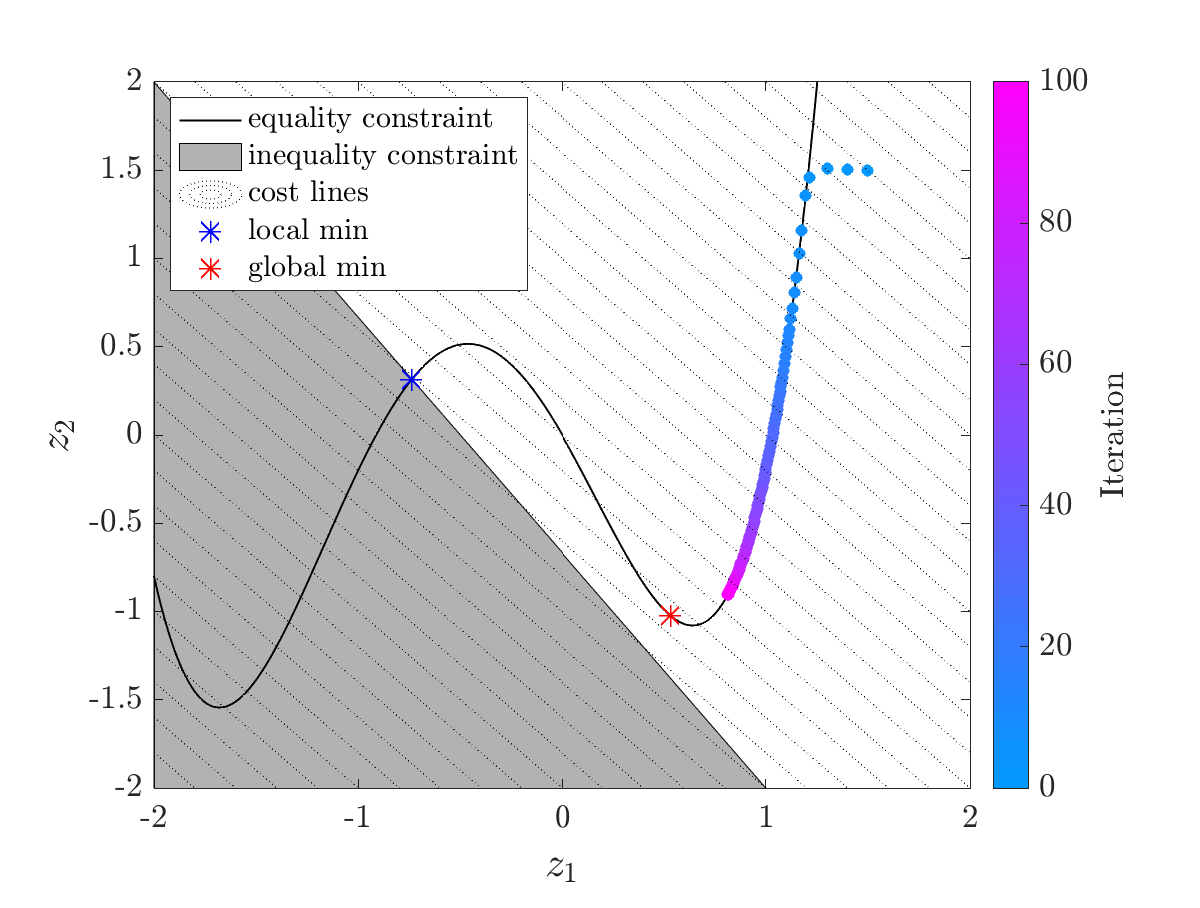
\includegraphics[width=0.33\textwidth]{figs/acc_toy_problem}} 
\subfloat[Relative error solution.\label{fig:toy_prob_soln_b}]{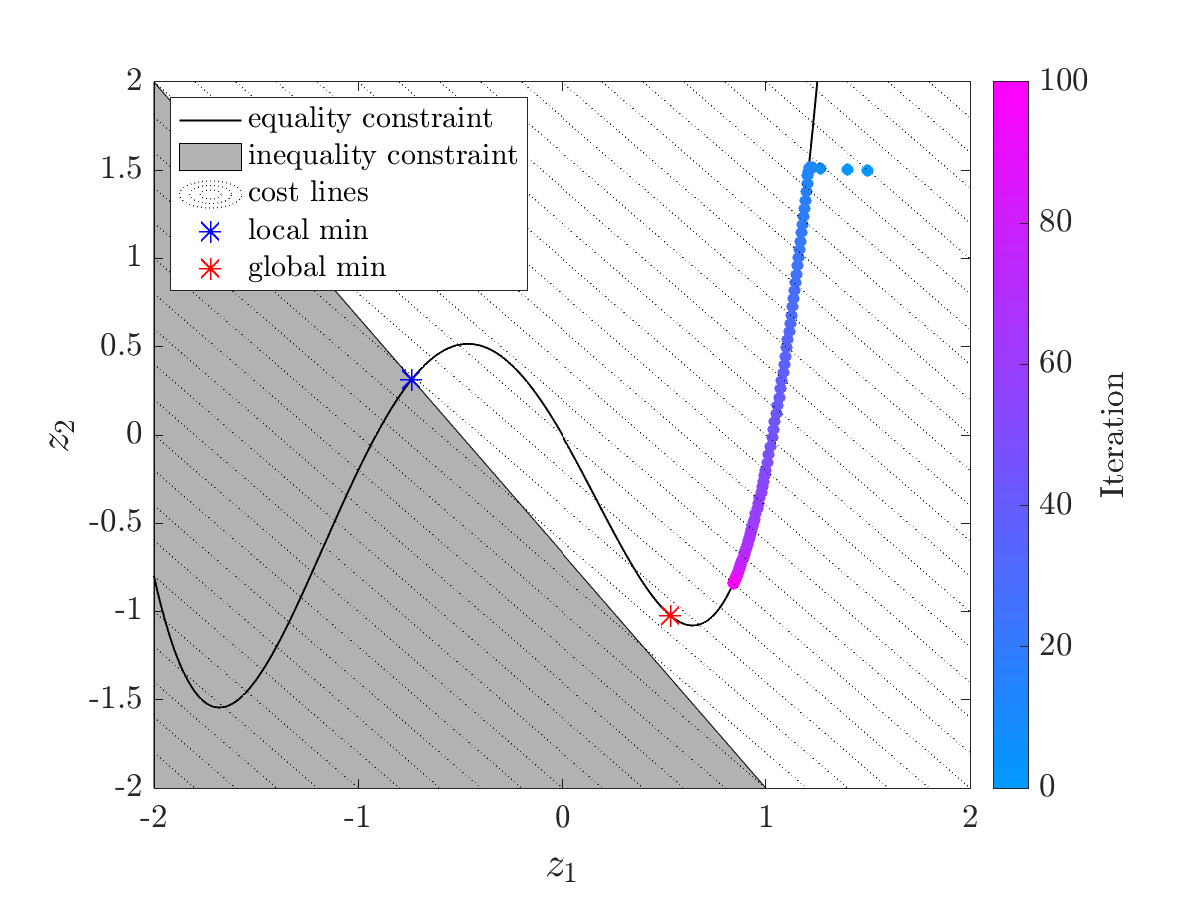
\includegraphics[width=0.33\textwidth]{figs/acc_toy_problem_relerr}} 
\subfloat[The performance metric $\pmet$. Color regions correspond to Figure~\ref{fig:scp_updates}.\label{fig:toy_prob_soln_c}]{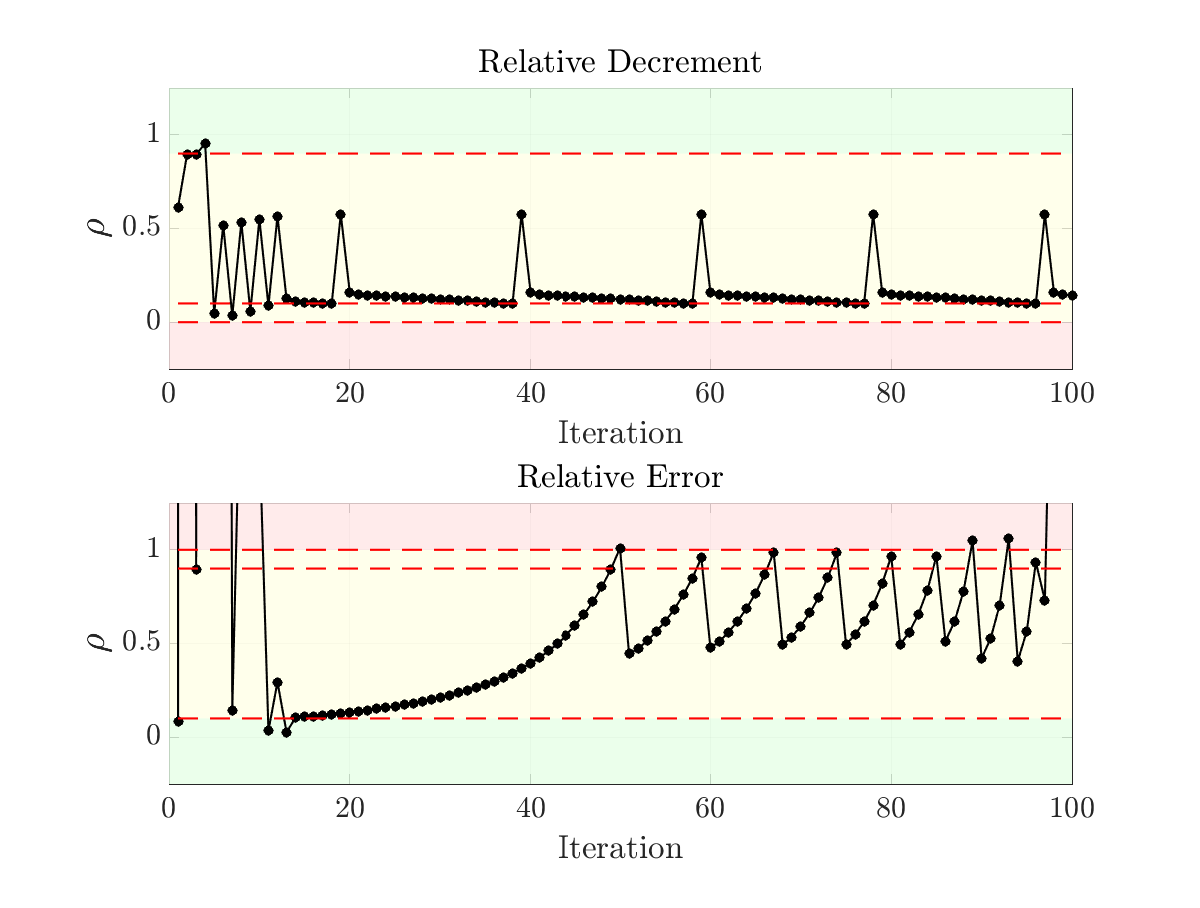
\includegraphics[width=0.33\textwidth]{figs/acc_toy_problem_rho}}
\caption{Solutions to Problem~\eqref{eq:toy_prob_cvx} across 100 iterations showing the crawling phenomenon.}
\label{fig:toy_prob_soln}
\end{figure*}

% \subsubsection{Discussion}

It is important to recognize the nuances of this toy example correctly and resist the temptation to draw overly general conclusions from it. For other choices of initial condition, the crawling phenomenon is avoided. For example, convergence to the local minimum from an initial reference in the shaded gray region is quite rapid, often terminting in ten or fewer iterations. There are, however, relatively large regions in the upper-middle and upper-right of the area plotted in Figure~\ref{fig:toy_prob_soln} from which the phenomenon is observed. We are merely pointing out that the crawling phenomenon \textit{can} happen, not that it \textit{will}. 

Moreover, it is obvious for this toy example that (i) the crawling phenomenon is occuring and (ii) that it occurs away from either minimum. This is only obvious because we know exactly where each minimum is (i.e., we can plot the cost lines and constraints). The trouble, in general, is that this is not possible. Higher dimensional non-convex problems for which no analytical solution is known do not permit the same observations that are obvious for this toy problem. The crawling phenomenon is effectively unobservable in the more challenging problems for which SCP methods are typically implemented on. Does slow progress mean that we have reached a local minimum? No. Arriving at a local minimum indeed implies that adjacent iterates will be close together (in the sense that $\|\z^*-\zb\|$ is small), but the converse is not necessarily true. 



% % introduce two ways of computing the progress metric; dJ/dL and dL/L. Both are susceptible to creeping.
% \begin{itemize}
% \item introduce the creeping phenomenon, provide a graphical description
% \item include an example of what this can look like
% \end{itemize}


\section{POSSIBLE REMEDIES: HYBRID ALGORITHMS}

\begin{itemize}
\item discuss possible remedies; if we know we have a feasible start, what can we do?
\item soft trust region methods?
\end{itemize}

\section{CONCLUSIONS}


% \addtolength{\textheight}{-12cm}   % This command serves to balance the column lengths
                                  % on the last page of the document manually. It shortens
                                  % the textheight of the last page by a suitable amount.
                                  % This command does not take effect until the next page
                                  % so it should come on the page before the last. Make
                                  % sure that you do not shorten the textheight too much.

%%%%%%%%%%%%%%%%%%%%%%%%%%%%%%%%%%%%%%%%%%%%%%%%%%%%%%%%%%%%%%%%%%%%%%%%%%%%%%%%



%%%%%%%%%%%%%%%%%%%%%%%%%%%%%%%%%%%%%%%%%%%%%%%%%%%%%%%%%%%%%%%%%%%%%%%%%%%%%%%%



%%%%%%%%%%%%%%%%%%%%%%%%%%%%%%%%%%%%%%%%%%%%%%%%%%%%%%%%%%%%%%%%%%%%%%%%%%%%%%%%
% \section*{APPENDIX}

% Appendixes should appear before the acknowledgment.

% \section*{ACKNOWLEDGMENT}

% The preferred spelling of the word ÒacknowledgmentÓ in America is without an ÒeÓ after the ÒgÓ. Avoid the stilted expression, ÒOne of us (R. B. G.) thanks . . .Ó  Instead, try ÒR. B. G. thanksÓ. Put sponsor acknowledgments in the unnumbered footnote on the first page.



%%%%%%%%%%%%%%%%%%%%%%%%%%%%%%%%%%%%%%%%%%%%%%%%%%%%%%%%%%%%%%%%%%%%%%%%%%%%%%%%

\bibliographystyle{ieeetr}
\bibliography{references}


\end{document}
